\documentclass[12pt]{report}
\usepackage{graphicx}
\usepackage{algorithm}
\usepackage{algorithmic}
\usepackage{keystroke}
\usepackage{pdfcomment}
\usepackage{gensymb}

\newcommand{\note}[1]{\raisebox{0pt}[0pt][0pt]{\pdfcomment[open=true]{#1}}}

% [dme] reordered these document definitions - title, author, date -
% if they sit here, they can potentially use the macros you include
% from packages
\title{Avoiding the Dark Side}
\author{
        Leslie Chisholm \\
                Department of Computer Science\\
}
\date{\today}

\begin{document}
\maketitle

\begin{abstract}
This is the paper's abstract \ldots
\end{abstract}

\tableofcontents
\listoffigures\
\listofalgorithms
\chapter{Introduction}
The city of Dunedin is well known for being a dark and cold city because of the hills surrounding the centre of the city that shade large areas in the winter months. This project set out to discover the amount of sunlight Dunedin receives and present the data in a user friendly manner.\\

\section{Goals}
The goals of this project were research and implement a sunlight projection model for the city of Dunedin. There are two parts; an interactive three-dimensional display to show point in time distribution of sunlight over Dunedin and a data aggregator to augment the display with computed measures of sunlight coverage over time ranges.\\

\section{Chapter outline}
Chapter two focuses on how physical data was gathered from the environment, the methods used to convert them into a representation usable for the project and the accuracy that was obtained in these measurements. Chapter three looks at the interactive three-dimensional viewer built to display the distribution of sunlight over Dunedin in real-time and its implementation using OpenGL and JOGL. Chapter four is about the data aggregator, which accurately calculates the amount of sunlight an area receives, how the data it calculates can be explored and the results generated.\\

\section{Background Information}
\subsection{OpenGL and JOGL} 
To create the viewer and allow it to be used in an interactive method the Java OpenGL (JOGL)\cite{JOGL} libraries are used. JOGL is a wrapper library that exports the OpenGL application programming interface (API) to the Java programming language. OpenGL or Open Graphics Library is a cross platform API for writing applications that use two and three dimensional computer graphics. The project uses version 2.0 of the OpenGL libraries for access to programmable shaders and buffer objects and will be able to run on any graphics hardware that supports OpenGL 2.0.\\

\note{Does `Background' normally sit in the introduction chapter? In a PhD thesis it would usually be chapter two. The problem with having it here is that the chapter outline comes after it. In most theses I've seen (these are not 480 project reports though) only the introduction text would come before the chapter outline. Hmm ok I've moved it to be after the chapter outline. I don't think a whole chapter could be taken up with background information}


\chapter{Physical Data}
To describe how shadows are cast over Dunedin physical elevation models and mathematical models of the sun's position are required. In this chapter the digital elevation model of Dunedin and the algorithmic model of the sun's position will be described and checked for accuracy.\\

\section{Elevation Data}

\begin{figure}
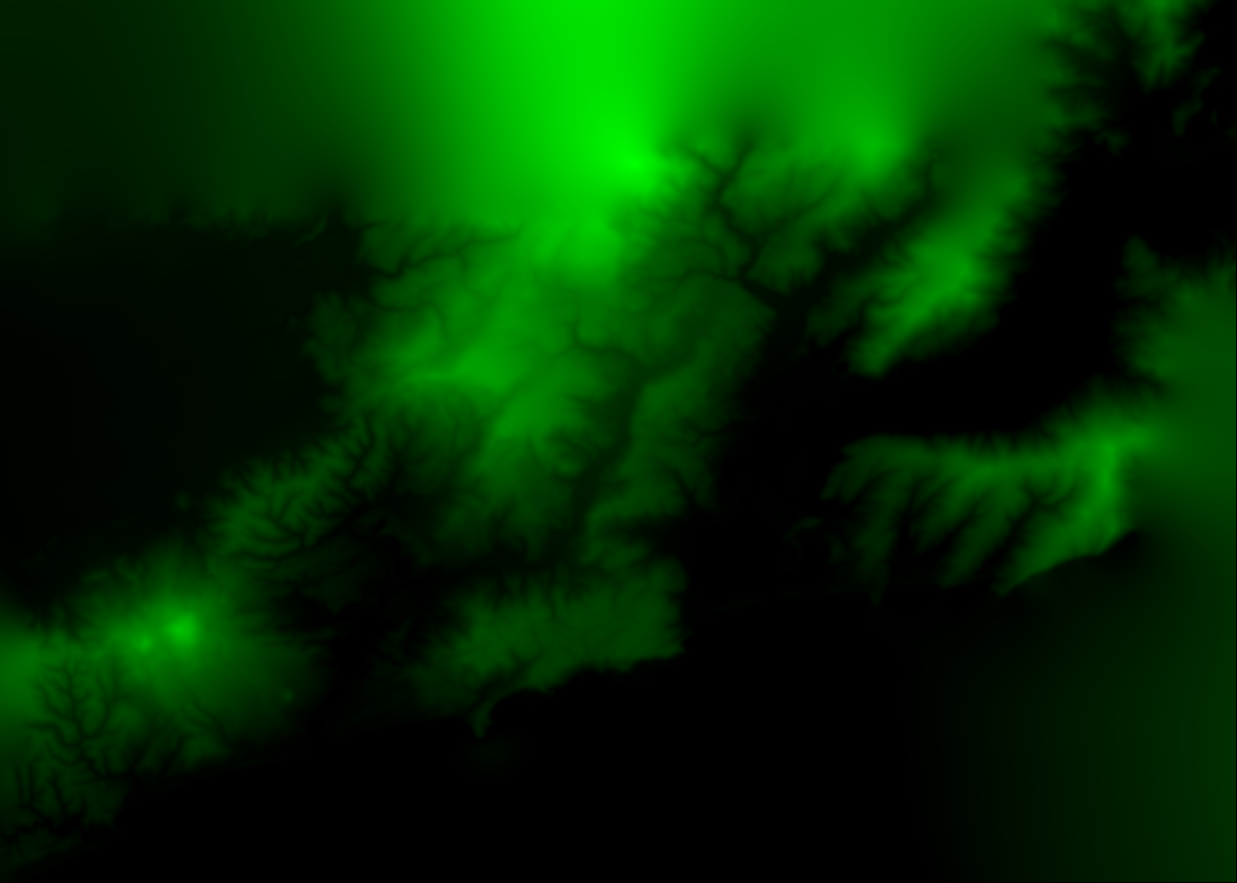
\includegraphics[scale=0.25]{height.png}
\caption{A Height Map generated from the data with low points dark and high points bright}
\label{image:elevation}
\end{figure}

The height data for Dunedin was collected from the surveying department of the University of Otago. The data contains a map with a width of 1237 points and a height of 881 points and covers most of general Dunedin from South Taieri to the top of Pine Hill. The data is encoded as a 1237x881 text file of decimal pointed numbers that represent the height above sea level in metres of that point. The resolution of the data is 15 metres between points.\\

From figure~\ref{image:elevation} it can be seen that there are areas that are less accurate where the data is approximated and smoothed out, such as the hills west of the Leith Valley and around Cape Saunders. The definition between what is in water and what is not also gets complicated when dealing with areas of reclaimed land like South Dunedin and the height data does not contain a fixed value for the water height.\\

\begin{figure}
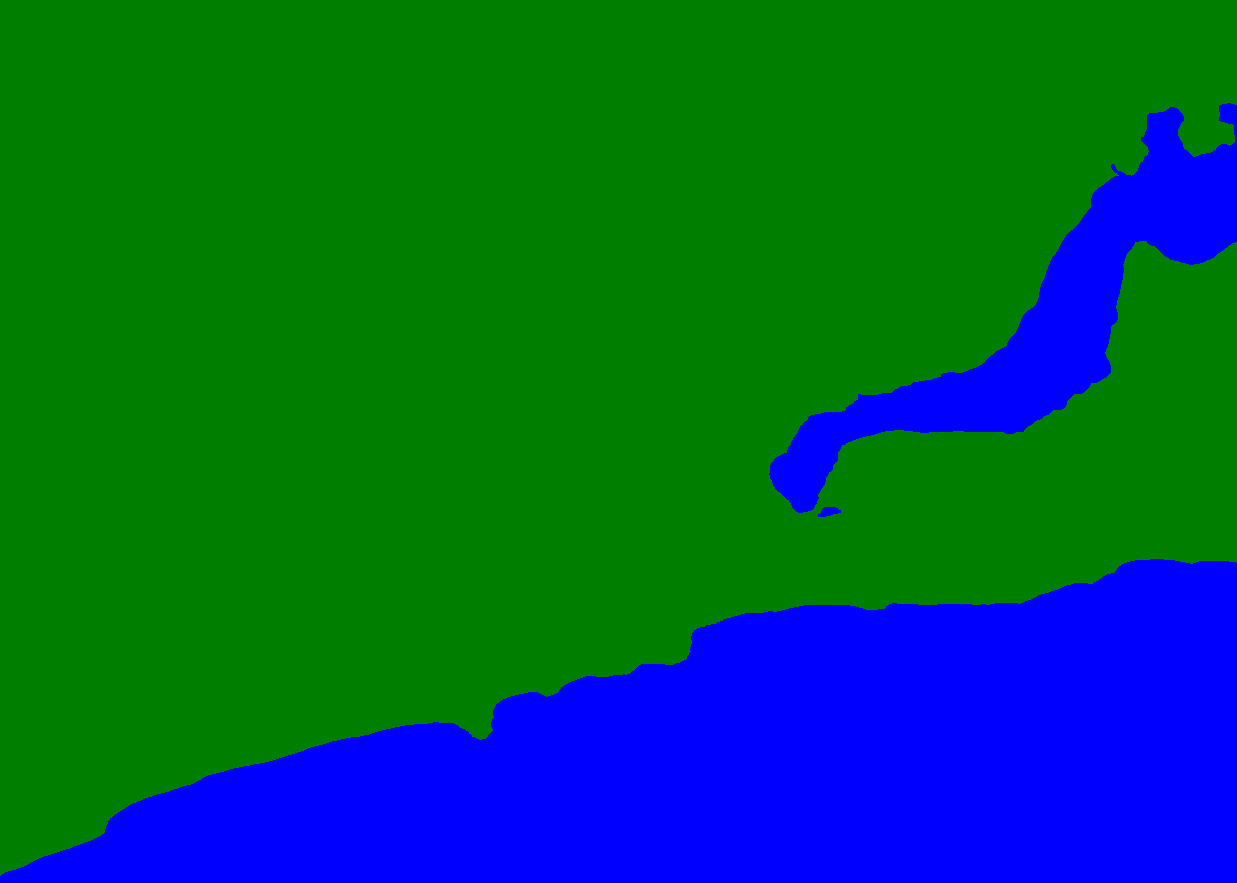
\includegraphics[scale=0.25]{terrain.png}
\caption{Water texture}
\label{image:overlaytexture}
\end{figure}
To work around the lack of definition of what is at water level and what is not, an image was generated (see figure~\ref{image:overlaytexture}) with the areas of water coloured a strong blue (RGB 0,0,255). The image is overlayed on the height data map when being used in the viewer with a 1:1 mapping of height points to image pixels to show what areas of land are in water. The areas of the height data that fall in the water are clamped to a height of 0.1 because the shape and depth of the ocean floor is of no use to the project.\\

\subsection{Accuracy}
To test the accuracy of the height data a global positioning system (GPS) was to be used to check the accuracy of the height points however this turned out to be infeasible because the accuracy of the GPS's height data was far lower than expected and to inaccurate to be included in the project. A GPS is rated to be accurate to approximately +/- 15 metres 95\% of the time\cite{gpsaltitude}. The inaccuracies were observed when standing at sea level with a GPS and getting results approximately 10 metres higher than the current position.\\

The best way to confirm the accuracy of the height data would be to compare it to other geographical data sources. Before going to the surveying department for the height information other sources were tried. The Shuttle Radio Topography Mission (SRTM)\cite{srtm} was a near-global scale project by NASA to generate topographical maps and includes all of New Zealand at a resolution of 30 metres. An old version of ARC GIS was provided by Geoff Wyvill containing topographical information of New Zealand, unfortunately the software to read the topographical maps was quite old and could not be run on any of the computers in the department.\\

\subsection{Future Work}
Unfortunately time constraints meant that there was not enough time to explore other height data sets.
 Given more time these data sources could be thoroughly explored and a larger collection of geographical data collected and utilised within the project, allowing the user to examine a larger area.

\section{Sun}
To generate shadows over the representation created of Dunedin the sun's current position has to be calculated accurately using a given time and geographical position.\\

\subsection{Calculating the Position of the Sun}
To calculate the position of the sun code from the RedShift project\cite{redshift} was used to ensure that the code had been previously tested. Code from other projects were examined, such as the solar positioning libraries for Java\cite{javasunlib} however the algorithms used in this library, the PSA\cite{psa} and SPA\cite{spa} algorithms, have the unfortunate downside that they do not work for areas in the Southern Hemisphere and modifying the algorithms used in their papers are outside the scope of the project.\\

To calculate the position of the sun the current Julian Date, solar declination and hour angle must be calculated. The Julian date is calculated by converting the current system UNIX time (seconds past January 1st 1970) into the current Julian Date (days since January 1, 4713 BC).
The hour angle is the angle between the plane of the Earth and the plane of the sun at a given time and is zero when the sun is directly above the Earth (solar noon). Calculating the hour angle can be done using the current longitude and Julian time. Solar declination is a measure of how many degrees North or South of the equator that the sun is when viewed from the centre of the earth and can be calculated by the current time. Using these calculations and the current latitude the sun's current azimuth and elevation can be easily computed.\\

The code modified from the RedShift library are the solar.c and solar.h files, which are taken from javascript code by U.S. Department of Commerce, National Oceanic \& Atmospheric Administration\cite{usnoaa} and is based on equations from Astronomical Algorithms\cite{astronomicalalgorithms}. \\

Redshift is only capable of calculating the altitude of the sun, so many (6 to be exact) different calculations for the azimuth were tried from multiple different sources. The most accurate calculation for finding the solar azimuth was found at the University of Southern California's Architecture Site\cite{solarazi}. Integrating the azimuth calculations into the rest of the code was simple using the calculations already present in the RedShift code to calculate the solar declination and hour angle.\\

\subsubsection{Time}
In calculating the position of the sun the current time must be known. Java's built in GregorianCalendar class was used to keep track of the current date/time, handle changes in daylight savings time and update the time. The method getSystemTimeMillis() was used when calculating the position of the sun because it returns the current UNIX time in milliseconds.\\

When the sun goes down ($sun elevation < 0$) the time class's update method enters a while loop increments the time until the sun comes back above the horizon. It does this by jumping forward six  hours in time, because every night in Dunedin lasts for at least six hours, and then incrementing the time in one minute time steps testing the sun elevation at the new time. Once the sun elevation gets back to above zero the Time code breaks out of the loop and returns control back to the program that called it. Taking conrol of the time once the sun goes beyond the horizon prevents the program unnecessarily wasting time and ensures at every point in time the sun is shining on a least some part of the map. Originally code for calculating the sunrise and sunset times were going to be used to tell the time that it needed to jump forward or backward to avoid being in complete darkness, however this code was thrown away because the calculations for the sun rise and set were to inaccurate and difficult to implement .\\%sometimes doing things the easy way IS the best way.

%\subsection{Calculating the Sunrise and Sunset} %might leave this out
%Calculations of the sunset and sunrise times taken from \cite{sunrise} 

\subsection{Sun Accuracy}

\begin{figure}
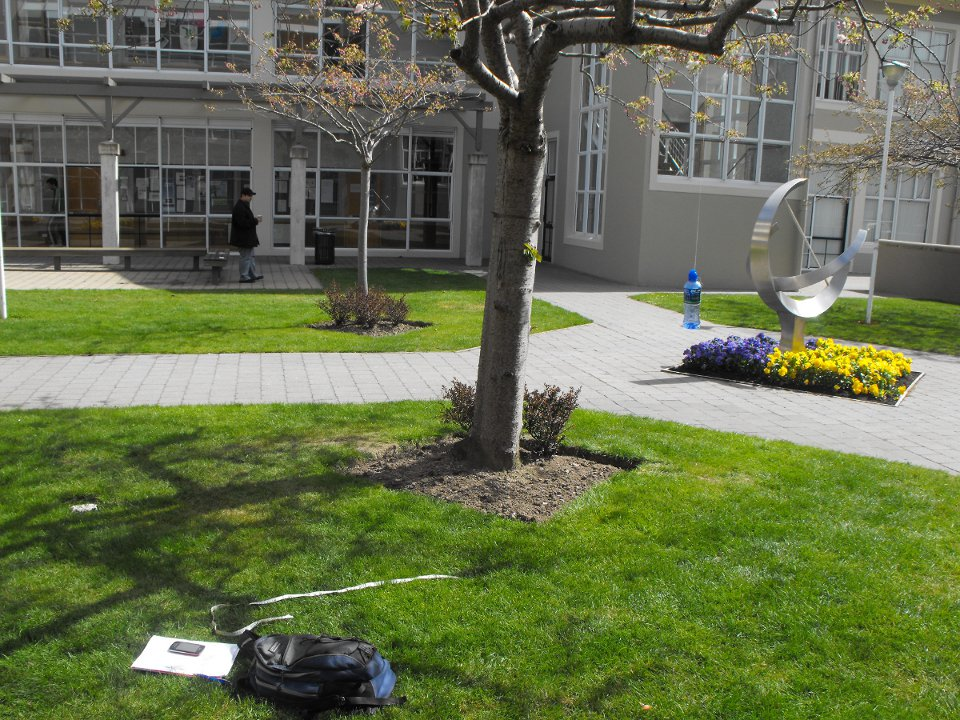
\includegraphics[scale=0.4]{contraption.jpg}
\caption{Device used to approximately calculate the position of the sun}
\label{image:sun-contraption}
\end{figure}

\begin{table}
\begin{tabular}{ | l | l | l | l  | l |}
\hline
Date Time & Sun Azimuth Website & Sun Azimuth Project & Sun Elevation Website & Sun Elevation Project\\ \hline
09:30 January 1st 2011 & 87.94462 & 87.9465 & 35.06 & 35.039\\ \hline
12:00 April 7th 2011 & 12.54622 & 12.5412 & 36.77 & 36.74896\\ \hline
16:00 June 14th 2011 & 314.4235 & 314.4227 & 7.243 & 7.1254\\ \hline
14:00 August 18th 2011 & 338.3437 & 338.34310 & 28.35 & 28.3225\\ \hline
15:19 October 4th & 321.1353 & 321.12823 & 41.72 & 41.698387\\ \hline
\end{tabular}
\caption{Calculated position of the sun using data scraped from satellite-caculations.com\cite{solarpos}}
\label{table:websun}
\end{table}


The accuracy of the sun was tested by comparing the results from the algorithms used in the project and by other sun position calculators and by creating a device to calculate the position of the sun at the current time. Using the solar position calculator from satellite-caculations.com\cite{solarpos} the solar altitude and azimuth at 15:19 on October 4th is 321.1353 and 41.72 degrees(including atmospheric refraction). Observing figure~\ref{table:websun} it can be seen that the results generated by the sun code in the project accurately resembles that generated by other code, even without taking atmospheric refraction into account.\\

A rudimentary device seen in figure~\ref{image:sun-contraption} was used to calculate the physical position of the sun by finding the angle between north and the shadow shadow cast by the device and the length of the shadow created compared to the length of the device. The device is made up of a piece of string tied to a weight and is hung from above to ensure that the device is pointing towards the centre of the Earth. The azimuth was recorded using a magnetic compass and modified to true north by applying Dunedin's magnetic declination (the angle between magnetic north and true north) of approximately 24.8\degree east. Data was taken from this device at three different times on the 5th of October from outside the Opheo building.\\

\begin{table}
\begin{tabular}{ | l | l | l | l | l}
\hline
Time & True Sun Azimuth & Sun Azimuth Calculation & True Sun Elevation & Sun Elevation Calculation\\ \hline
13:08 & 15.8 & 7.027 & 44.09 & 48.4507 \\ \hline
14:47 & 344.8 & 330.967 & 40.376 & 45.1352\\ \hline
13:12 & 337.8 & 322.955 & 43.914 & 42.766\\ \hline
\end{tabular}
\caption{Calculated position of the sun using real data}
\label{realsun}
\end{table}

From figure~\ref{image:realsun} it can be seen that the calculation differences are quite different between the physical position of the sun and the calculated position of the sun. The difference is caused almost entirely by the errors in gathering the physical data. Firstly the mobile phone compass used to find the azimuth of the sun is highly inaccurate giving values that are +/- 40\degree for the same direction. Secondly the device created to measure the elevation of the sun had a tendency to oscillate in the wind and lastly the surface the length of the shadow was being measured on was not perpendicular to the device. All of the elevation calculations are within 5\degree and the azimuth calculations are within 20\degree which is within the possible margin or error caused by these effects. Compensation for these errors is outside the scope of this project and thus the physical calculations are shown as an estimated value.\\

\chapter{Viewer}

\begin{figure}[h]
\centering
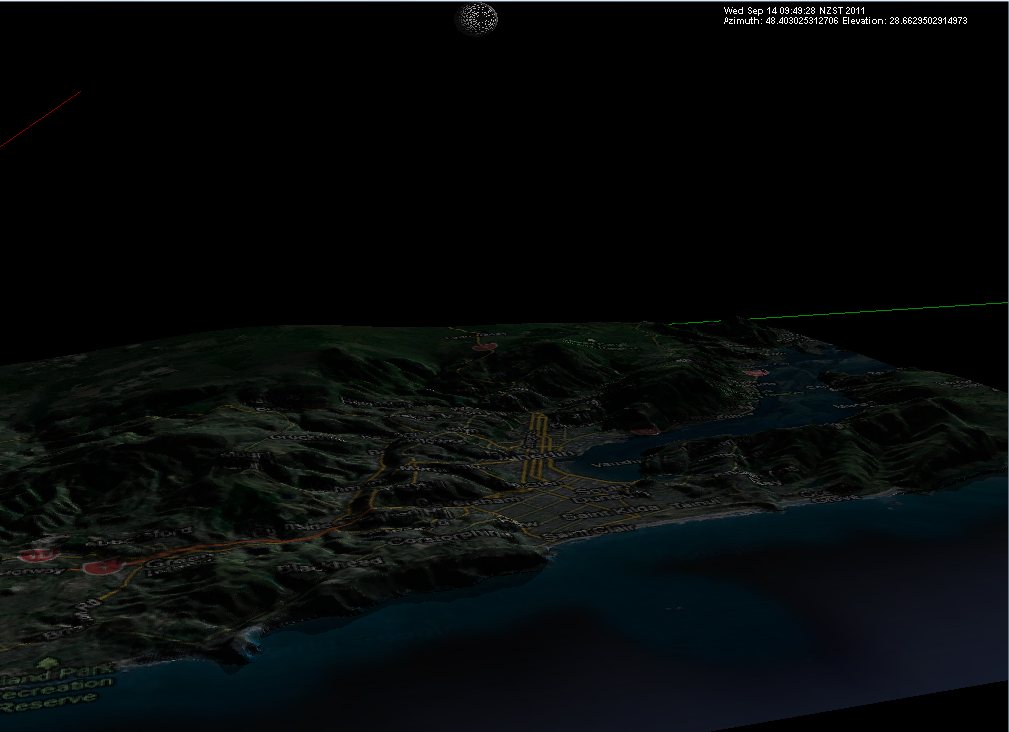
\includegraphics[scale=0.4]{viewer.png}
\caption{A screenshot of the viewer looking down at Dunedin}
\label{image:viewer}
\end{figure}

The viewer is an interactive three-dimensional simulator of the Sun moving over Dunedin. It allows the user to view shadows cast by the sun over the varying landscape. It exposes the ability to run in two different modes; shadow-mapping mode, where OpenGL shadow maps are used to generate shadows, and aggregator shadowing mode, where the shadow data from the aggregator is used to calculate shadows. This chapter will focus mainly on how OpenGL and shadow mapping are used to draw and shadow the scene.\\

\section{Drawing the elevation data}
Geographical height data is drawn by the viewer using OpenGL. After the height data has been gathered by the program OpenGL buffer objects are created to store the vertex position, colour, texture coordinates and vector normals. Buffer objects allow sending the data to be drawn directly to the graphics cards local memory where it can be redrawn and updated quickly without resending the information. Due to the large number vertices present in the height data and the static nature of the data, using buffers to store the vertex data lowers the number of graphics hardware calls significantly in comparison to using the fixed function pipeline and increases the speed of the viewer.\\

\section{Drawing the textual information}
In figure~\ref{image:viewer} there is a box in the top right hand corner that shows the current time, solar azimuth and solar elevation. Drawing this data is done using the built in JOGL TextRenderer class and a two-dimensional orthographic projection matrix.

\subsection{Overlay Data}
A map overlay is drawn over-top of the scene to show major roads, points of interest and terrain information. The map was taken from Google Maps\cite{gmaps} and scaled to be the exact width and height of the height data. The overlay information is drawn into the scene by colouring the 

\section{Shadows and lighting}

The viewer is capable of showing shadows generated using OpenGL shadow maps and shadows calculated using the aggregator. Shadows, lighting and textures are drawn onto the scene using vertex and pixel shaders. Diffuse and specular lighting are performed by calculating the dot product of the vertex normals with the position of the sun. Shadow lighting is implemented by using shadow mapping to test whether a given pixel can be seen by a light source. Textures, which are only used by the aggregator shadows, are drawn in the fragment shader using the built in GLSL texture2D function to get the colour at a given vertex from the texture.\\

\subsection{Shadow Maps}
Shadow mapping is a method of quickly generating shadow information from a three-dimensional view which sacrifices accuracy for speed and ease of implementation. Shadow mapping works by storing the depth values of a scene from the lights view into an off-screen frame buffer object and testing the depth component of each pixel in the scene against the stored depth value at that point. If the . In implementing shadowing mapping code was copied from Fabian Sanglard's website\cite{shadowb} and modified to work using Java and JOGL.\\

The accuracy of a shadow map is limited by the resolution of the off-screen buffer and the accuracy of the depth buffer. The resolution of the shadow map used in the viewer is 8 times that of the scene and so is reasonably accurate at the expense of some speed.

\section{Visual Comparison Between the Viewer and Dunedin}
\begin{figure}[h]
\centering
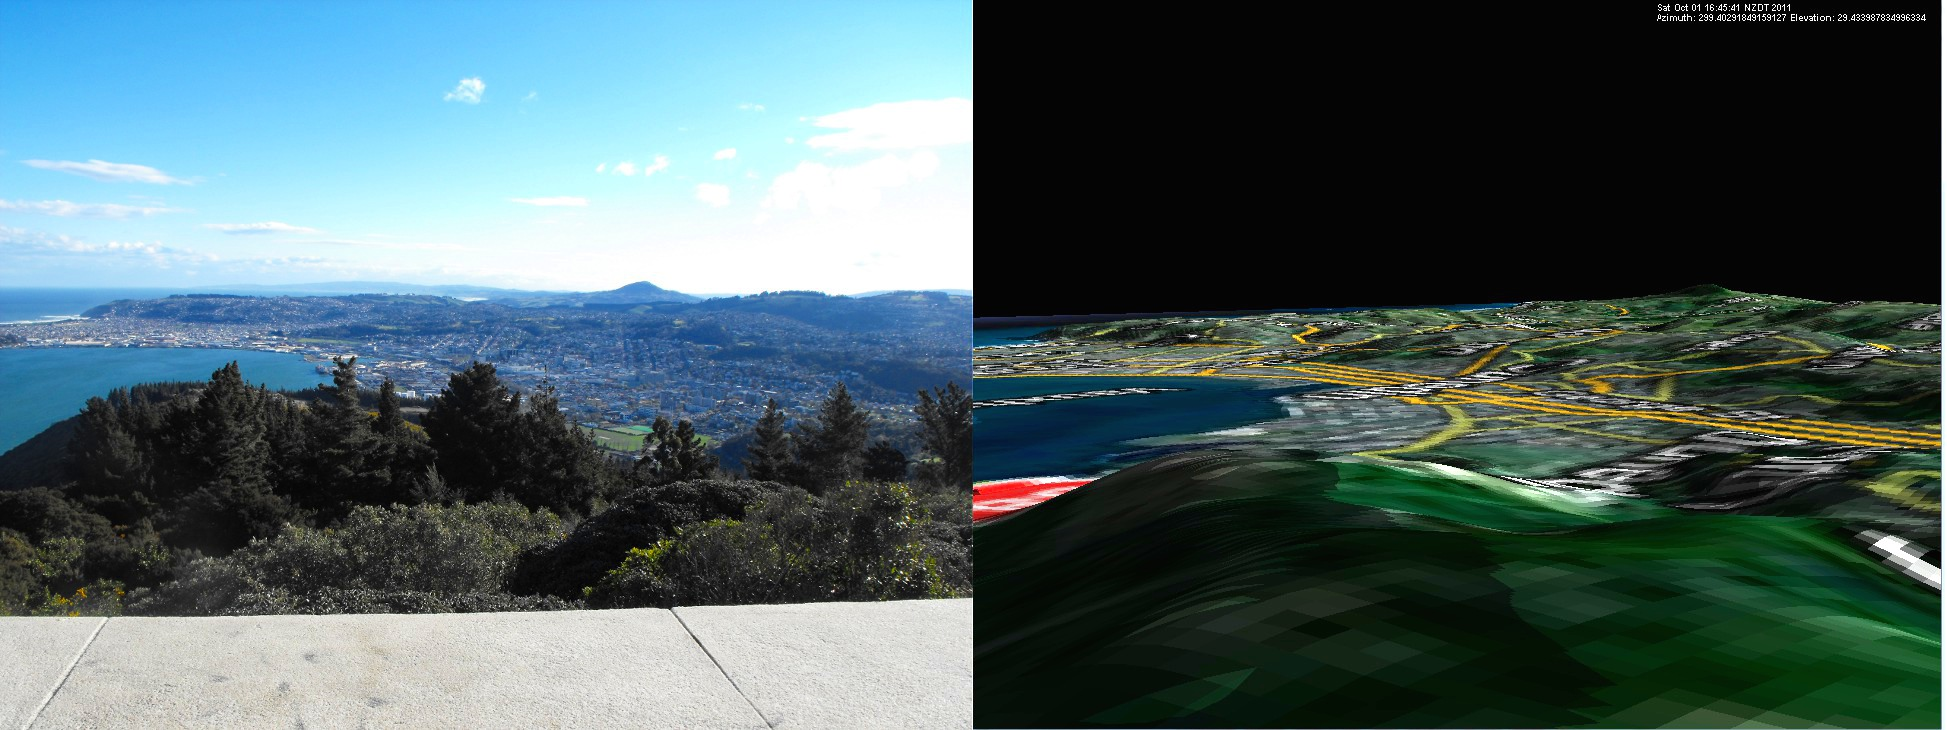
\includegraphics[scale=0.2]{realvsviewer.jpg}
\caption{A camera image taken from signal hill at 16:45 on September 28th 2011 and the same image generated in the viewer}
\label{image:realvsviewer}
\end{figure}

In figure~\ref{image:realvsviewer} it can be seen that the scene generated by the viewer from the top of signal hill is very similar to that of an actual image. All of the major geographical features of Dunedin can be made out and similar shadows are present in both images.

\section{Usage}
To run the viewer firstly the JOGL libraries must be installed and set up to work with the installed Java runtime library. Running the OpenGL code requires graphics card that fully supports OpenGL. See the controls below for an idea of how to run it. Command line parameters are not taken
\subsection{Control}
\texttt{w} $\rightarrow$ Move forward\\
\texttt{s} $\rightarrow$ Move Backward\\
\texttt{a} $\rightarrow$ Strafe Left\\
\texttt{d} $\rightarrow$ Strafe Right\\
\texttt{f} $\rightarrow$ Toggle Wireframe mode\\
\texttt{p} $\rightarrow$ Print the current 3D coordinates to stdout\\
\texttt{=} $\rightarrow$ Increase the time speed by one second\\
\texttt{-} $\rightarrow$ Decrease the time speed by one second\\
\texttt{0} $\rightarrow$ Stop time\\
\texttt{h} $\rightarrow$ Move camera position to signal hill\\
\texttt{m} $\rightarrow$ Toggle between aggregator shadows and shadow mapping\\
\texttt{g} $\rightarrow$ Start/stop the aggregator updating\\

Mouse drags can be used to rotate the camera up,down,left,right. For example if the user wishes to look to the right they would click and drag the mouse right and the camera will move once they let go of the mouse.

\section{Future Work/Scrapped Ideas}
Instrumenting the viewer to run a loop based on a script passed into the viewer was always on the tables as something that would be nice to implement if there was enough time. This would have allowed the program to give a quick demonstration of how it can be used and what values can be gathered without looking through the documentation.

\chapter{Aggregator}

The aggregator is designed to calculate whether a portion of land is in shadow or not more accurately then using OpenGL methods such as shadow mapping. It can be run as a standalone program where it outputs targa image files and comma separated value files for the number of sunlight seconds received over a period of time or as part of the viewer where it can be used to expose it's accurate shadow calculations.

\section{Cleary's Algorithm for Calculating Shadows}
To calculate whether a given point is in shadow or not a modified version of Cleary's algorithm is used, see algorithm~\ref{alg:shadow-calculation} for a full description. Cleary's algorithm was originally used for fast spacial subdivision however it works equally well in raytracing a light ray from a point through a two-dimensional grid of points like the one present in the elevation data. For each point the light ray travels from the source to the sun through each grid square it meets until it reaches the end of the grid. At each grid line intersection the height at that point is compared to the height of the sun along the direction vector between the starting point and the sun, if the direction vector's y value multiplied by the current length along the vector is less than the height at that point then it is said to be in shadow, otherwise it continues on the direction vector until the end of the grid is reached or another point triggers it to be in shadow.

\begin{algorithm}[h]
\caption{Calculate whether a given x,y point on the map is in shadow or not}
\label{alg:shadow-calculation}% and a label for \ref{} commands later in the document
\begin{algorithmic}           % enter the algorithmic environment
\STATE $directionToSun \Leftarrow sun.directionVector$
\STATE $heightAtPoint \Leftarrow map.getHeight(x,y)$
\STATE $tdx \Leftarrow 1 / directionToSun.x$
\STATE $tdy \Leftarrow 1 / directionToSun.y$
\STATE $xPostion \Leftarrow x$
\STATE $yPosition \Leftarrow y$
\WHILE{$xPosition < map.width$ and $yPostion < map.height$ and $xPosition \geq 0$ and $yPosition \geq 0$}
	\IF{$(height at xPostion,yPostion$ and $ABS(MAX(tdx,tdy))) > directionToSun.y\times ABS(MAX(tdx,tdy))$}
		\RETURN{$In Shadow$}
	\ENDIF
	\IF{$ABS(tdx) < ABS(tdy)$}
		\STATE $dx \Leftarrow 1 / directionToSun.x$
		\IF{$tdx > 0$}
			\STATE $xPosition \Leftarrow xPostion + 1$	
		\ELSE
			\STATE $xPosition \Leftarrow xPostion - 1$	
		\ENDIF
		\STATE $tdx \Leftarrow tdx + dx$
	\ELSE
		\STATE $dy \Leftarrow 1 / directionToSun.y$
		\IF{$tdy > 0$}
			\STATE $yPosition \Leftarrow yPostion + 1$	
		\ELSE
			\STATE $yPosition \Leftarrow yPostion - 1$	
		\ENDIF
		\STATE $tdy \Leftarrow tdy + dy$		
	\ENDIF
\ENDWHILE
\RETURN{$Not In Shadow$}
\end{algorithmic}
\end{algorithm}

\section{Integration into the viewer}
The aggragator output can be run in the viewer if the use aggregator and generate aggregator texture switches are turned on. The aggregator works in the viewer by generating a texture out of the current shadow information that is white for not in shadow and black for not in shadow. By placing the texture over the map of Dunedin aggregator shadows can be observed on the terrain. Because the aggregator code uses different shader code to the viewer the overlay images and shading are not drawn on the scene.

\section{Picking the areas to scan}
The aggregator uses the overlay image seen in figure~\ref{image:overlaytexture} to select which points to scan. Any area that is coloured blue is counted as water and any area that is a solid black colour is ignored. This allows the user to specify specific areas of Dunedin that they may want to explore (by painting them black) and running them through the aggregator faster than when it has to go through all the points. It is unlikely that a user would want to find the amount of sunlight an area of sea receives (unless they farm plankton?) and for this reason any areas in water are also ignored by the aggregator.

\section{Comparison to OpenGL Shadow Mapping}
\begin{figure}[h]
\centering
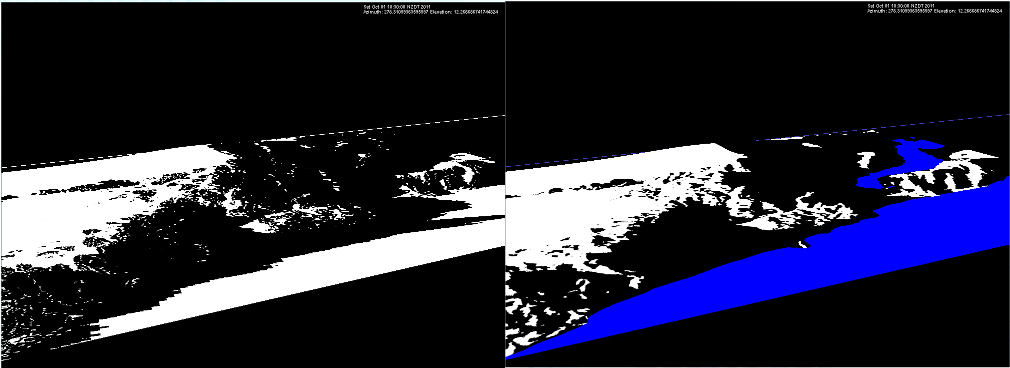
\includegraphics[scale=0.6]{aggregatorvsshadowmapping.png}
\caption{A side-by-side screenshot comparison of shadowing using shadow mapping (left) and the aggregator (right)}
\label{image:aggregatorvsshadowmapping}
\end{figure}

Shadow maps are noticeably less accurate at calculating shadows then the aggregator is. In a side-by-side comparison it can be seen that shadows generated by shadow mapping have noticeable aliasing and calculation errors. Aliasing around the edge of occurs in the shadow map when the angle between the sun and the map of Dunedin approaches 180\degree and the shadows begin to gen very long. Self-shadowing is also a problem with shadow mapping and can only be fixed by increasing the accuracy of the depth buffer (
which considerably slows down shadow calculations). Neither of these problems arise in the data aggregator because of the accuracy gained by ray-tracing the area between the shadow and the sun and checking for intersections. The aggregator pays for this accuracy by running slower than real-time (approximately 7 seconds between calculations for a slow machine and 2.5 on a fast machine)compared to the shadow maps which run at >30 calculations/second with a dedicated graphics processor.\\

\section{Output}%would be good to get a pretty picture of what area receives the most sun here
When the aggregator is run as a standalone program a targa image file and/or a comma separated value file can be output from the program. These files can output the amount of sunlight seconds received over some period of time.\\

\section{Optimisations}
The aggregator can be run faster than by naively checking every height point by checking for shadows around the edges of a small area of land. If there is no shadow present at any of the edges and the area is reasonably flat then it is safe to assume that all of the points within that region will not be in shadow. The aggregator uses a square area of 10 points which it scans around the outside edge of for shadows, if no shadow is found then all of the points within the square are set to be not in shadow.\\

\subsection{Speed increase}
To test the effect of the optimisations the data aggregator was run 1000 times on the whole of Dunedin (ignoring only water) between the times of 08:00:00 and 17:59:24 on October 1st 2011, with the average time in milliseconds it took to run the aggregator recorded at each time. On a 1.9GHz AMD Dual Core Turion processor the optimised code took an average of 6800.486 milliseconds and the unoptimised code took 15977.598 milliseconds to calculate all of the shadows at a given time. Using 2.66 GHz Intel Core i7 920 processor the optimised code took an average of 1147.176 milliseconds and the unoptimised code took 2551.007 milliseconds to calculate the shadows. Using the optimised code increased the speed by a factor of 2.35x on the 1.9GHz processor and 2.19x on the 2.66GHz processor.\\

\subsection{Other Methods}
The code does not necessarily need to be optimised to speed it up. With multi-core processors becoming more common on computers multi-threading the aggregator code to take advantage of more than one processor at a time would give scalable performance increases. The way the testing for shadows is implemented is easily threadable by spawning a thread for every block in the array that needs to be processed.\\

%Implementing this could even be programmed in massively multi-threading languages such as OpenCL 

\note{Good. Well expressed, too. Perhaps mention that there are more general forms of this optimisation strategy, but that there will be a cross-over point between the efficiency gained by not computing shadow rays against the extra effort in running the optimisation algorithm.}


\section{Data Gathered}
By running the aggregator for the whole year it was seen that suburb x managed to receive the highest amount of sun... %this is currently running. I will put an image on here showing the distribution of sun on the o

\section{Future work}
Multi-threading the code, further optimisation and comparing it to other methods of accurately calculating shadows.
\chapter{Conclusion}
In the end the project was able to do x well and didn't do y as well as expected.


\bibliographystyle{abbrv}
\bibliography{480}

\end{document}
